\chapter{Application Domain}
This chapter aims to define the required functionality of both the server and the client side of the solution. Furthermore, this chapter describes which types of persons could be using the solution. 


\section{Interaction Design}
\subsection{PACT - designing for people}\label{pact}
%!TEX root = ../../Master.tex
When designing an interactive system it is important to think about the people using it. The people are a part of the interactive system and therefore it is important to make sure that the design fits the people. In~\cite{benyon2013designing} PACT analysis is presented as a framework for thinking about design situations. To help with the design being human centred, the designer needs to understand the four parts of the analysis: It is important to understand the different kind of people using the system, since they have different prerequisites for using a system. The activities that people want to undertake are equally important, as it says a lot about the way the system will be used. The designer needs to think about the context, the location and organisation, the system will be used in, which provide information about how the system should operate. Lastly the designer should consider the features of interactive technologies and how to incorporate them in the design.

\begin{figure}
  \centering
  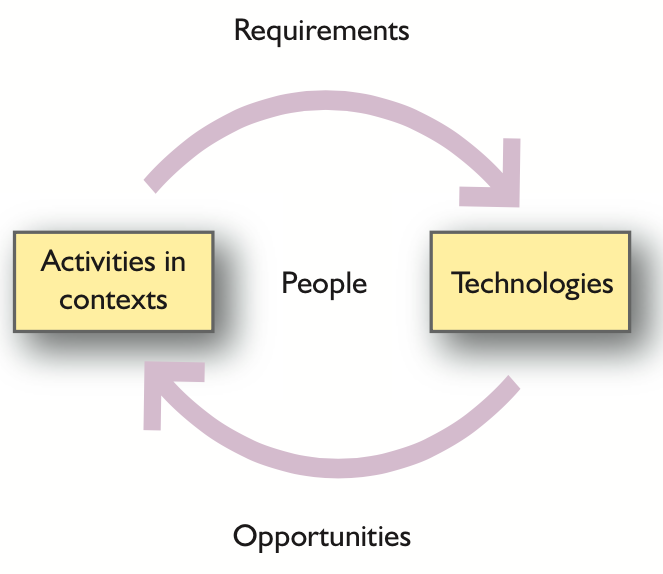
\includegraphics[width=0.5\linewidth]{pact-overview.png}
  \caption{The relationships between activities, contexts, people and technologies in PACT. From~\cite{benyon2013designing}}
  \label{fig:pact-overview}
\end{figure}

It is also important to understand the relationship between activities and technologies. \Cref{fig:pact-overview} shows how the activities people are doing will influence the requirements for technologies. This will create new technology that will change the activities people will be doing with the technology.

It is the variety of requirements that is found during the PACT analysis, that can make designing systems difficult. Therefore, an analysis of the four core elements of PACT will be conducted.


\subsection{People}
\label{sub:pact_people}

The system is used by people who go to bar-like environments, and are possibly intoxicated. At bar-like environments, music is central to the atmosphere, and a lot of people are interested in having their music tastes accommodated. Different people exhibit different behaviour in these social contexts, some may clique together when using a social system and some may be afraid of stigmas when using it. To use the system, a smartphone is required, and some people may be unable or afraid \chnote{uddyb hvorfor} to use their smartphone.

\subsection{Activities}
\label{sub:pact_activities}

Usage of the system requires the user to interact with their smartphone or similar device. Firstly the user must install the application on their device. The installation process should not take a long time, or else the user might forget about the application. When the user is checked-in, the current playlist of the venue will be displayed. The transition from the check-in to the playlist screen should occur in less than 100 milliseconds as to not frustrate the user. From the playlist screen the user can vote on a track. Finding which track to vote for should not be a complex action, as this is an expected frequently done action.

\paragraph{New or improved activities}
The system introduces a possibility of requesting a track to be played at the venue, without having to ask the administrator. This eases work load on administrator, which might be busy serving beverages to a customer. It also eases the process of requesting a track by not having to get up if sitting and splitting from one's group or partner, which may lead to a more time spend together. The system might change the behavior of the users and serve as topic of discussion, possibly an icebreaker. These changes in activities should be considered when designing the system.

\subsection{Context}
\label{sub:pact_context}

This system can be used at places where many people wants to listen to music, but does not have an efficient method \chnote{påstand, uddyb} of determining which tracks to listen to.

A dark environment with a lot of noise is common in bars/pubs. As people are often dancing in this environment, active use of smartphones is not recommended\chnote{why}. Also, usage of smartphones in these kind of environments often cause anti-social behaviour. \chnote{kilde ville være super nice :)}

\subsection{Technologies}
\label{sub:pact_technologies}

The system runs on a host computer with an audio system connected and a business license for Spotify. \chnote{meget specific?} This host computer is located at the installation site.

For users to operate this system a smartphone with internet connection and adequate battery life is required. \chnote{ved vi alle de ting? hvis det skal ikke skal være i retrospekt}
When designing the system, different smartphones and their characteristics have to be considered.

\subsection{Summary}
\label{sec:pact_summary}

As the people using the system are possibly intoxicated and in contexts of meeting and talking to other people, by speech, it is considered rude and anti-social to neglect the interactive to using a smartphone. Other ways of interacting with the system could be considered, or to minimize the time spend on smartphone usage. Therefore the system must be \textbf{quick}* \footnote{Frequent and determined users might access the system often with a already known task for the system, making them capable of communicating a request of system very quickly, the system should sought to not be the limiting factor in this process.} and \textbf{easy to navigate and use}, by focusing on providing a small and effective set of functionalities. Pervasive computing is a significant part of the system, and therefore battery saving on these mobile device is of concern, therefore a requirement of the system is to \textbf{minimize power consumption} as result of usage of the system, by not doing extensive computing on the clients side.

Also in the context of the system, the users might be dancing... \chnote{maybe relevant}

The PACT analysis provide us with these requirement:
\begin{itemize}
  \item Should be quicker than the user
  \item Easy to use and navigate - Few but effective functionalities
  \item No extensive computations on the client
\end{itemize}


\subsection{Persona}
\frnote{ret}
The people that use a system can be represented by personas. This is done in order to ensure the PACT elements are centered in the design process\kanote{Hvad menes der her?}. Personas are general profiles of different types of users. A persona is a concrete representation of a fictitious person. Personas help the designer by having a specific end user in mind, preventing them designing the system for themselves. Personas are developed through the understanding process and through undertaking a PACT analysis. A part of the persona is a short story of the person trying to achieve a goal using the system in a specific context~\cite{benyon2013designing}.

As part of this project, a persona was made, based on the interviews which were conducted.%\cref{interviewbruger}.
This is Camilla, an average user of the system.

\subsubsection{Camilla}
\begin{figure} [h]
  \centering
  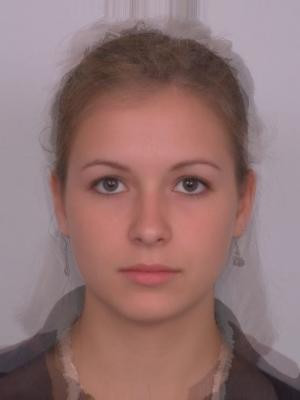
\includegraphics[]{Images/average.jpg}
  \caption{Picture associated with the persona \enquote{Camilla}. Copyright the Face Research Lab. Used with permission.}
  \label{fig:camilla}
\end{figure}
\noindent\textbf{Basic information}
\begin{itemize}
\item 25 years old
\item Medical student
\item Employed in an elderly care center
\item In a relationship with Keith
\item She loves meeting new people
\item When going out she likes to visit small places that allow socialisation
\item Volunteered in Red Cross Uganda
\end{itemize}

It is Friday afternoon and Camilla is planning to meet some of her fellow students at a bar. Camilla and her friends get together after they are finished at school and go to a café to grab a sandwich. After dinner, Camilla takes out her smartphone and checks openPlaylist. Camilla can see that some of her favourite songs are being played at White Hart, and they agree to go there. Upon arriving Camilla checks in via the application. She immediately notices on the screen behind the bar that the queue is filled with songs she dislikes. She now uses the application to request and upvote other songs that she would like to be played. Some other people at White Hart agree on Camilla's choices and they too upvote these songs. On the screen in the bar Camilla can see some of the other people that upvotes her songs and later in the evening she meets them and they talk about all the nice music they have in common. Camilla and her new and old friends party all night long and drink a lot of beer.

\section{Use Cases}\label{usecase}
\subsubsection{Actors}
There are two actors of this system is the administrator, a bartender or a bar owner in charge of the music, and the guest, wanting to request and affect the music. From this 

\begin{table}[h]
\begin{tabular}{lcc}
\hline
                   & \multicolumn{1}{l}{\textbf{Actor}} & \multicolumn{1}{l}{} \\
\textbf{Use case}  & Administrator                      & Customer             \\ \hline
play music         & \checkmark                         &                      \\
stop music         & \checkmark                         &                      \\
next track         & \checkmark                         &                      \\
add restriction    & \checkmark                         &                      \\
remove restriction & \checkmark                         &                      \\
check out          &                                    & \checkmark           \\
check in at venue  &                                    & \checkmark           \\
vote               &                                    & \checkmark           \\
cancel vote        &                                    & \checkmark           \\ \hline
\end{tabular}
\end{table}

\actortable{Administrator}{
    \textbf{Purpose:} A person in charge of the music, wants to be able to have control over the system, what kind of music is being enqueued and what is currently playing.

    \textbf{Characteristics:} Has a preference or a theme of music that the individual is following, set by the organisation or the invidual itself.

    \textbf{Possible usage:} adds restrictions, removes restriction, play music, stop music, play next track.
}

Diagram of possible usage, see \cref{fig:UsageAdmin}
\begin{figure}
  \centering
  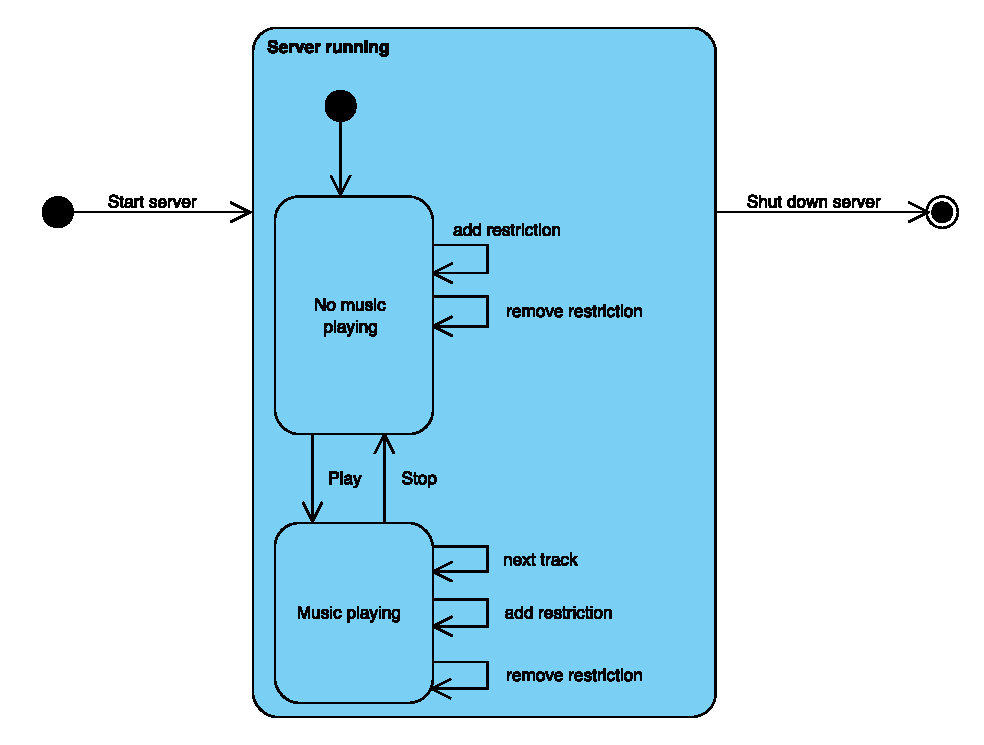
\includegraphics[width=0.7\linewidth]{Images/UsageAdmin.pdf}
  \caption{Usage for a administrator}
  \label{fig:UsageAdmin}
\end{figure}

\actortable{Guest}{
    \textbf{Purpose:} Wants to listen to a preferred track at the venue, the individual is visiting.


    \textbf{Characteristics:} Music preferences may differ from the administrator set of preferences, or allowed themes of music, at a specific venue.

    \textbf{Possible usage:} Check in at venue, check out, vote for
    track, cancel vote.
}
Diagram of possible usage, see \cref{fig:UsageUser}
\begin{figure}
  \centering
  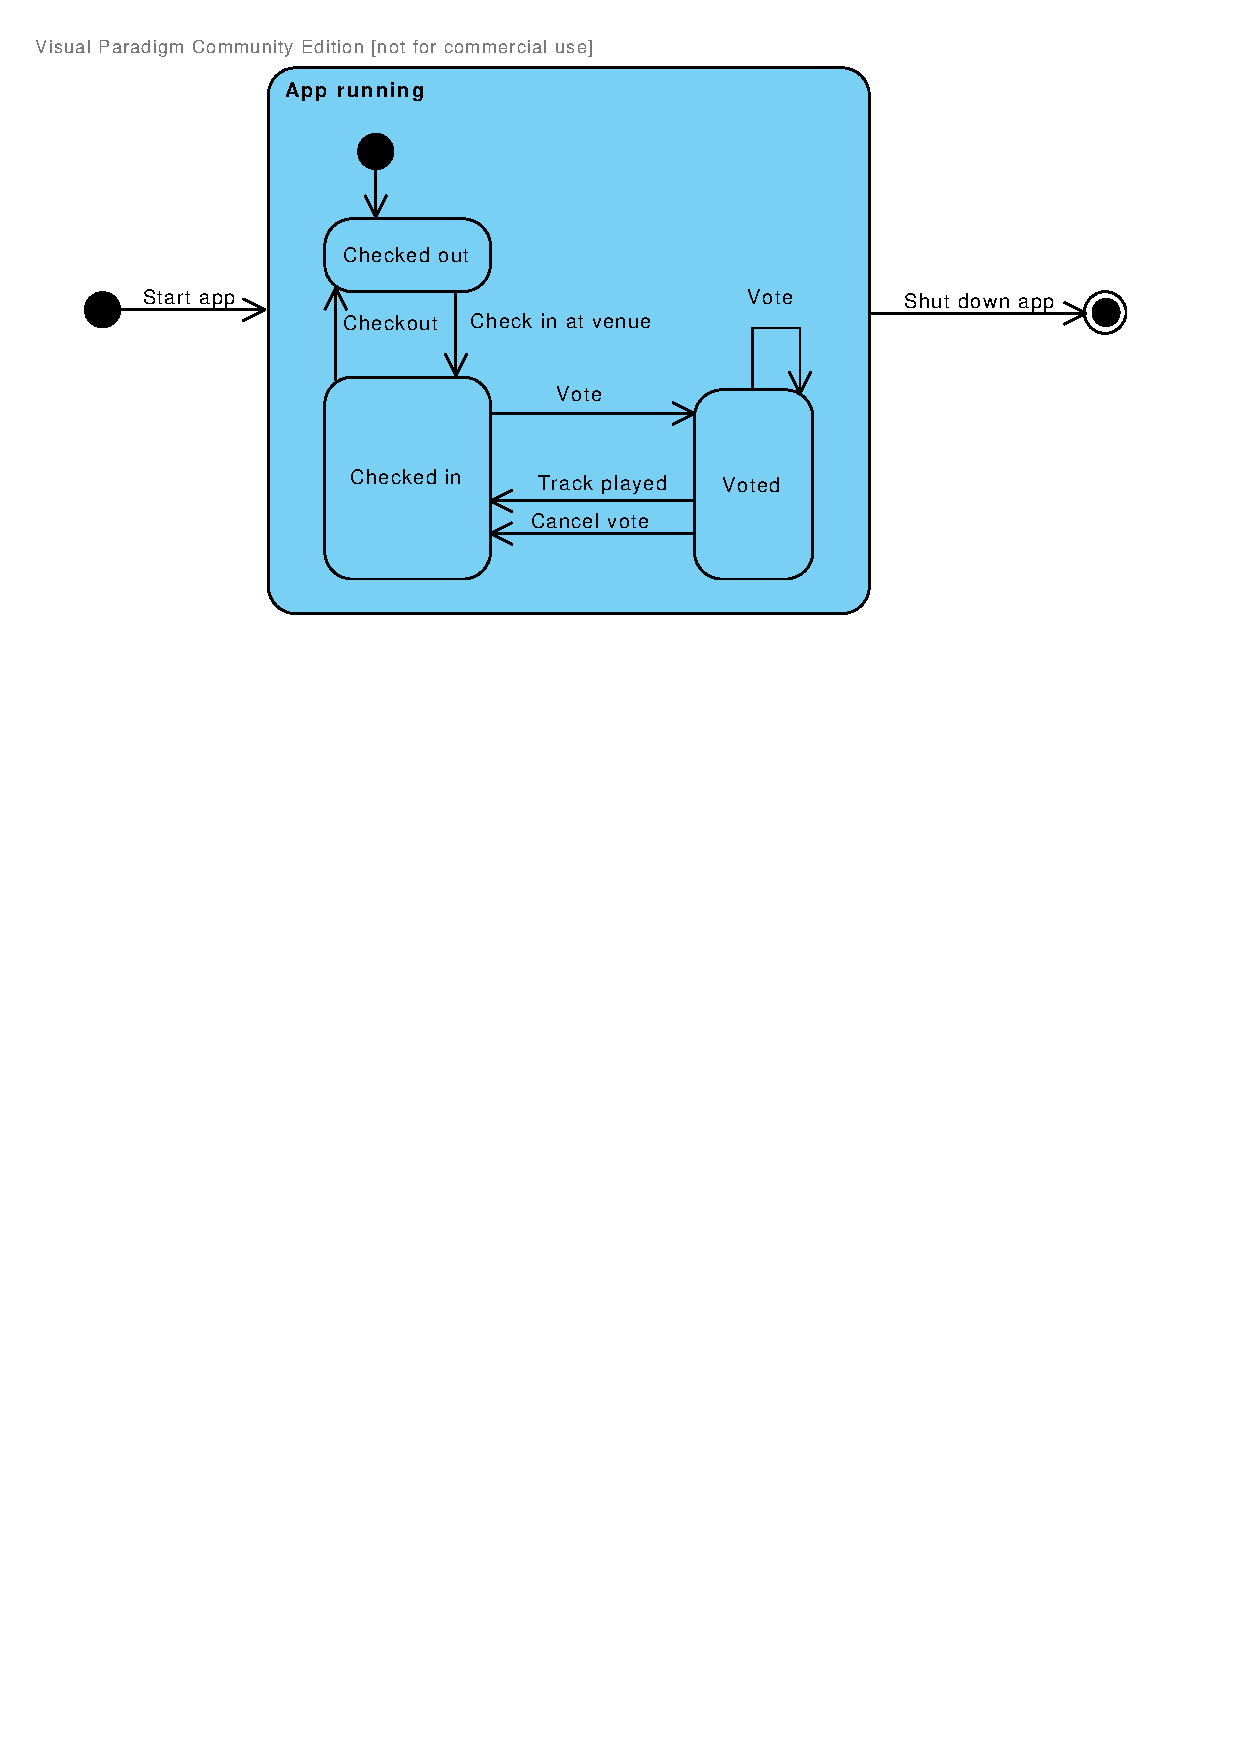
\includegraphics[width=0.7\linewidth]{Images/UsageUser.pdf}
  \caption{Usage for a guest}
  \label{fig:UsageUser}
\end{figure}


\section{Functions}
As part of the analysis of the application domain an analysis of the functions are needed. It is done in order to get an understanding of what the system should do. A function is something that make the model usable by the user and supports they use cases. There are three different kinds of functions:

\emph{Update} functions are functions that are triggered by an event in the problem or application domain that then needs to update the state of the model. Update function is used to keep the model up to date with reality.

\emph{Signaling} functions are triggered by changes in the model. They notify the actors or do a direct action in the problem domain.

\emph{Read} functions are functions that makes the model readable by the outside. It is used by an actor when he need updates from the model in the system.

\emph{Compute} functions are similar to  read functions but instead of just reading the model they do some extra computation. They might also read different places in the model and combining them with some computation.

In \cref{table:functionlist} is a table of function from the system. The functions was made based on Use cases and the systems definition. The table also includes the complexity of the functions. This is a subjective assessment made in collaboration with the users of the system. It tells how difficult a function is to develop. Most functions can can be specified with just a name but some of the more complex functions needs to have a detailed specification.

\begin{table}[h]
\begin{tabular}{lll}
\hline
\multicolumn{3}{c}{\textbf{Social music playing}} \\ \hline
Filter                         & Medium & Compute \\
Create filter                  & Simple & Update  \\
Read filter                    & Simple & Read    \\
Update filter                  & Simple & Update  \\
Delete filter                  & Simple & Update  \\
Get current playlist           & Simple & Read    \\
Change song votes              & Simple & Update  \\
Play something on the speakers & Medium & Signal  \\
Change playing state           & Medium & Update  \\
Song vote                      & Medium & Update  \\
Get next song                  & Complex & Compute \\
Noget med søg                  &        &         \\ \hline
\end{tabular}
\caption{Function list}
\label{table:functionlist}
\end{table}

\frnote{Specification of complex functions}

